\label{modelagem}

Neste capítulo  será apresentada uma proposta de modelagem matemática . . .


\section{Procedimentos Experimentais}
\label{Procedimentos Experimentais}


Para realizar a análise de viabilidade econômica, são necessários alguns valores previamente calculados e apresentados anteriormente, nesta seção, em  conjunto com as informações apresentadas no Quadro \ref{quadro6}.

\begin{quadro}[!ht]
  \centering
  %\setlength{\tabcolsep}{60pt}
%\renewcommand{\arraystretch}{1}
\caption{Dados a ser considerados para a simulação. }
%\resizebox{\linewidth}{!} {
\begin{tabular}{|c|c|}
\hline
Consumo   atual           & 400,00 kWh    \\ \hline
Custo de disponibilidade  & 50,00 kWh     \\ \hline
Simultaneidade            & 30,00\%       \\ \hline
Energia gerada pelo SFV    & 400,00 kWh    \\ \hline
Iluminação pública        & R\$ 27,00     \\ \hline
Tarifa                    & R\$ 0,75      \\ \hline
Poupança anual            & 6,50\%        \\ \hline
Taxa   DI             & 8,00\%       \\ \hline
Aumento da tarifa         & 8,00\%        \\ \hline

Investimento sem financiar & R\$ 17.124,90 \\ \hline
\end{tabular}
\label{quadro6}

Fonte: Produzido pelo autor
\end{quadro}



Para comparar as técnicas escolhidas desta tese, foi utilizado o Erro Relativo (ER), ou seja:
%
\begin{equation}
E_r=\frac{|x_i-\overline{x}|}{\overline{x}}.\label{eqerrorelativo}
\end{equation}
%
onde: $E_r$ é o erro relativo, $x_i$ é o valor imputado, e $\overline{x}$ é o valor real.

Na Equação \ref{eqerrorelativo} é realizada a divisão do erro absoluto, entre o valor original e o imputado, em módulo, pelo valor atual para encontrar o percentual do erro relativo de cada um dos registros imputados. Para obter o valor final para analisar a eficácia, é realizada a média entre todos os $E_r$ encontrados dentro de cada cenário para cada técnica executada, sendo definida como melhor aquela que possuir a menor média.


Na Tabela \ref{tabela:execucoesmediana_cenario_1} é apresentado o percentual de $ER$ de cada uma das oito execuções da técnica, e na Figura~\ref{fig-execucoesmediana_cenario_01} é apresentado o gráfico da evolução dessas execuções.


\begin{table}[!h]
\caption{Sequência de Execuções Mediana para o Cenário 1.}
\label{tabela:execucoesmediana_cenario_1}
\centering
\begin{tabular}{cc}
\hline
\thead{Execução} & \thead{Erro Médio} \\
\hline
1   &   1,58\% \\
2   &   1,58\% \\
3   &   1,61\% \\
4   &   1,59\% \\
5   &   1,54\% \\
6   &   1,50\% \\
7   &   1,50\% \\
8   &   1,54\% \\
\textbf{Média} & \textbf{1,56}\% \\ \hline
\end{tabular}
\end{table}



\begin{figure}[!h]
\centering
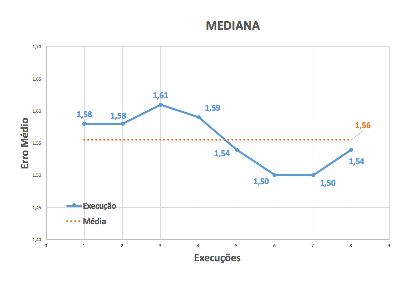
\includegraphics[scale=2.0]{imagens/execucoesmediana.eps}
\caption{Análise comparativa do $ER_{med}$ das oito execuções da Mediana.}
\label{fig-execucoesmediana_cenario_01}
\end{figure}
